\section{System Model}
\label{pbs:system_model}
This section outlines the system model on which the solution is built. Definitions for new concepts are introduced first, considering they will be used to describe the different components that consist of the system model. Later subsections explain in detail the different components and processes required for the prediction-based solution. We assume that all the transactions are well-formed and the scheduler is legal.

\subsection{Definitions}
\label{pbs:definitions}

\defCommitRate{cmt_rate}
\defEfficiencyRate{eff_rate}

\begin{definition}
\label{cat_bounds}
 (Categorization Thresholds) - categorization thresholds are upper and lower limits of both commit rate and efficiency rate that are used when categorizing transactions\footnote{The categorization bounds are static values that do not change throughout the system execution. Both the efficiency rate and the commit rate bounds are currently at 50\% creating full coverage of all transactions.}.
\end{definition}

% \begin{definition}
% \label{cat_threshold}
%  (Categorization Thresholds) - categorization thresholds are calculated within the categorization bounds (see Definition \ref{cat_bounds}) by using the Transaction Concentration Ratio (see Section \ref{sec:TCR}). The threshold values are dynamic and change depending on the execution environment but will not exceed the categorization bounds placed on that particular category. Categorization thresholds enforce the most accurate thresholds for the execution environment while allowing flexibility.
% \end{definition}

\begin{definition}
\label{transaction_categories}
(Transaction Categories) - Let $T$ = \{$T_{1}$, ... , $T_{n}$\} be a set of transactions and $C$ = \{$HCHE$, $HCLE$, $LCHE$, $LCLE$\} a set of category names. The mapping $\tau$ associates a category name with each transaction as follows:

\[ 
\tau : \textrm{$T_{i}$}\rightarrow
\left \{
  \begin{tabular}{cc}
  HCHE & if $C_{r}(T_{i}) > 0.5$ and $E_{r}(T_{i}) > 1$ \\
  HCLE & if $C_{r}(T_{i}) > 0.5$ and $E_{r}(T_{i}) \le 0.5$ \\
  LCHE & if $C_{r}(T_{i}) \le 0.5$ and $E_{r}(T_{i}) > 1$ \\
  LCLE & if $C_{r}(T_{i}) \le 0.5$ and $E_{r}(T_{i}) \le 0.5$
  \end{tabular}
\right \}
\]

{\normalfont In order to ensure correct lock techniques are selected, transactions cannot be simply characterized as good or bad based on their metrics. For example, a transaction $T_{1}$ may have a 100\% commit rate, but it may have a long execution time. A transaction with these characteristics should not be penalized when, in fact, it is a well behaving transaction. On the other hand, a transaction $T_{2}$ that has a 100\% commit rate and has an extremely short execution time should not be treated with the same priority as $T_{1}$. This is where certain of levels must be established to ensure the most appropriate selection is made.

In order to establish levels, a system of categories was put in place base on the metrics mentioned previously. The first categorization is based solely on the efficiency of the transaction. In this categorization, there are two attributes: \textit{high efficiency (HE)} and \textit{low efficiency (LE)}. A transaction that has been labeled as \textit{HE} is considered to execute with an efficiency in the upper 50\% of all transactions executed within the system\footnote{See Section \ref{pbs:cat_graph} and Section \ref{pbs:definitions} for more clarification}. The second attribute, \textit{LE}, is any transaction where its efficiency rate is in the lower 50\% of all transactions executed.

The second categorization that the levels are built on is based solely on the outcome of the transaction. These attributes are \textit{high commit (HC)} and \textit{low commit (LC)}, which are much more simple to define. A transaction with a \textit{HC} attribute has committed successfully over 50\% of executions (upper 50\% of all transactions). A transaction with an \textit{LC} attribute has failed over 50\% of its executions (lower 50\% of all transactions). This categorization correlates directly with the commit rate defined (see Definition \ref{cmt_rate}).

With these two categorizations and two attributes, a four-level system was devised in order to select appropriate lock types. The four categories devised are \textit{high commit-high efficiency (HCHE)}, \textit{high commit-low efficiency (HCLE)}, \textit{low commit-high efficiency (LCHE)}, and \textit{low commit-low efficiency (LCLE)}. Depending on the level in which the transaction has been placed, different lock types will be granted in order to perform concurrency control.}

\end{definition}

\begin{definition}
\label{cat_dominance}
(Transaction Category Dominance) - The Transaction Category Dominance is a pair, denoted as $C_{D} = (C,L)$, where $C$ is the set of transaction categories, and $L$ is a partial order of the categories such that:
 
\[\textrm{$HCHE > HCLE > LCLE$}\]
\[\textrm{$HCHE > LCHE > LCLE$} \]

\begin{figure}[h]
\captionsetup{justification=centering}
\centering % used for centering Figure

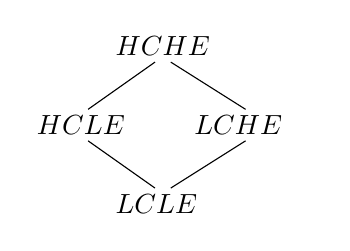
\begin{tikzpicture}
    % [list/.style={rectangle split, rectangle split parts=3,
    % draw, rectangle split horizontal}, >=stealth, start chain]
  \node[text width=1.5cm] at (3.8,5) {$HCHE$};
  \node[text width=1.5cm] at (2.8,4) {$HCLE$};
  \node[text width=1.5cm] at (4.8,4) {$LCHE$};
  \node[text width=1.5cm] at (3.8,3) {$LCLE$};
  \draw (3.55,4.8) -- (2.7,4.2);
  \draw (3.75,4.8) -- (4.7,4.2);
  \draw (3.55,3.2) -- (2.7,3.8);
  \draw (3.75,3.2) -- (4.7,3.8);
  
\end{tikzpicture}

% \caption{Web Service Environment with Scheduler} % title of the Figure
\label{fig:category_lattice} % label to refer figure in text

\end{figure}

{\normalfont Note that the categories $HCLE$ and $LCHE$ are not comparable. That is, we cannot establish a dominance relation between transactions in $HCLE$ and $LCHE$ categories.

However, in our model, we focus on reducing the need of compensation for aborted transactions. Therefore, we prioritize the commit property over the efficiency property. We introduce the dominance relation below in Table \ref{tbl:priority}.}

\[\textrm{$HCLE > LCHE$} \]
 
\begin{table}[h]
\captionsetup{justification=centering}
\centering
\begin{tabular}{l|c|}
\cline{2-2}
                                          & \multicolumn{1}{l|}{\textbf{Priority}} \\ \hline
\multicolumn{1}{|l|}{\textbf{HCHE}}  & I                                      \\ \hline
\multicolumn{1}{|l|}{\textbf{HCLE}}  & II                                     \\ \hline
\multicolumn{1}{|l|}{\textbf{LCHE}} & III                                     \\ \hline
\multicolumn{1}{|l|}{\textbf{LCLE}} & IV                                      \\ \hline
\end{tabular}

\caption{Category Priorities} % title of the Figure
\label{tbl:priority} % label to refer figure in text

\end{table} 

\end{definition}

% \begin{definition}
% \label{min_commit}
% (HCHE) - HCHE, acronym for High Commit High Efficiency, is a transaction categorization with categorization bounds (see Definition \ref{cat_bounds}) that involve a commit rate of 50\% and higher and a efficiency rate in the upper 50\% and higher as well (see Definitions \ref{cmt_rate} and \ref{eff_rate}). Table \ref{tbl:default_tmetrics} outlines all transaction categories.
% \end{definition}

% \begin{definition}
% \label{min_abrt}
% (LCHE) - LCHE, acronym for Low Commit High Efficiency, is a transaction categorization with categorization bounds (see Definition \ref{cat_bounds}) that involve a commit rate of 50\% and lower and a efficiency rate in the upper 50\% and higher (see Definitions \ref{cmt_rate} and \ref{eff_rate}). Table \ref{tbl:default_tmetrics} outlines all transaction categories.
% \end{definition}

% \begin{definition}
% \label{ext_commit}
% (HCLE) - HCLE, acronym for High Commit Low Efficiency, is a transaction categorization with categorization bounds (see Definition \ref{cat_bounds}) that involve a commit rate of 50\% and higher and a efficiency rate in the bottom 50\% and lower (see Definitions \ref{cmt_rate} and \ref{eff_rate}). Table \ref{tbl:default_tmetrics} outlines all transaction categories.
% \end{definition}

% \begin{definition}
% \label{ext_abrt}
% (LCLE) - LCLE, acronym for Low Commit Low Efficiency, is a transaction categorization with categorization bounds (see Definition \ref{cat_bounds}) that involve a commit rate of 50\% and lower and a efficiency rate in the bottom 50\% and lower as well (see Definitions \ref{cmt_rate} and \ref{eff_rate}). Table \ref{tbl:default_tmetrics} outlines all transaction categories.
% \end{definition}

%\begin{definition}
%\label{no_trend}
%(NO\_TREND) - NO\_TREND is a transaction categorization with categorization bounds (see Definition \ref{cat_bounds}) that include all %the outlining space that the previous four categories do not include. If the efficiency rate is less than or equal to 25\% then the %commit rate must be between 25\% and 75\% (see Definitions \ref{cmt_rate} and \ref{eff_rate}). If the efficiency rate is between 25\% %and 75\% then the commit rate includes all values ranging from 0\% to 100\%. Finally, if the efficiency rate is greater than or equal %to 75\% then the commit rate must be between 25\% and 75\%. Table \ref{tbl:default_tmetrics} outlines all transaction categories.
%\end{definition}

%\[
%\left \{
%  \begin{tabular}{ll}
%  
%  $E_{r}\le25\%$, & $25\%<C_{r}<75\%$ \\
%  $25\%<E_{r}<75\%$, & $0\%\le C_{r}\le100\%$ \\
%  $E_{r}\ge75\%$, & $25\%<C_{r}<75\%$
%  
%  \end{tabular}
%\right \}
%\]

\begin{definition}
\label{conflict_ops}
 (Conflicting Operations) - two operations are conflicting:

 \begin{enumerate}
   \item they are contained within two different transactions,
   \item both operations are operating on the same data item, and
   \item at least one of the operations is a WRITE
 \end{enumerate}

 \begin{example}
 \label{ex_conflict_ops}
  Let $o_{1}$ be a READ operation on data item $User ID$ in transaction $T_{1}$ and let $o_{2}$ be a WRITE operation on $User ID$ in $T_{2}$. These two operations are conflicting.
 \end{example}
\end{definition}

% \begin{definition}
% \label{conflict_trans}
%  (Conflicting Transactions) - two transactions are considered conflicting if they contain all of the following attributes:
 
%  \begin{enumerate}
%  \item both transactions contain conflicting operations (see Definition \ref{conflict_ops})
%  \item both transactions are contained within the same serializable schedule
%  \item and at least one of the transactions is categorized to abort
%  \end{enumerate}
 
%  \begin{example}
%  \label{ex_conflict_trans}
%   Using the transactions mentioned in Example \ref{ex_conflict_ops} let's say the serializable schedule $S_{1}$ contains   an interleaved execution of $T_{1}$ and $T_{2}$. These transactions are now considered conflicting.
%  \end{example}
% \end{definition}

% \begin{definition}
% \label{conflict_cat}
%   (Conflicting Categories) - conflicting categories are very much related to conflicting transactions (see Definition \ref{conflict_trans}) however this definition is concerned with the categories the transactions have been placed in rather than the transactions themselves. Two categories are said to be conflicting if they contain all of the following attributes:
  
%   \begin{enumerate}
%   \item both are contained within the same serializable schedule
%   \item and at least one of the categories is predicted to abort
%   \end{enumerate}
  
% Transactions of conflicting categories are not allowed within the same schedule within this solution.  
  
%   \begin{example}
%   For example, let's say we have transaction $T_{1}$ that has been placed in the category HCHE and transaction $T_{2}$ that has been placed in the category LCLE. These two categories are considered conflicting even if $T_{1}$ and $T_{2}$ are not considered to be conflicting transactions themselves.
%   \end{example}
  
% \end{definition}

% \begin{definition}
% \label{serial_sched}
%  (Serializable Schedule) - a serializable schedule is a non-serial schedule that can be converted to a serial schedule by interchanging non-conflicting operations (see Definition \ref{conflict_ops})

% \end{definition}

% \begin{definition}
% \label{casc_rollback}
%  (Cascading Rollback) - a cascading rollback occurs when two conflicting transactions (see Definition                     \ref{conflict_trans}) are interleaved within the same serializable schedule. The abort is cascading in the sense that an  abort must be issued for each transaction within the schedule that was dependant upon the transaction that issued the abort. This is needed to ensure a consistent state within the database.
 
%  \begin{example}
%  \label{ex_casc_rollback}
%   Using the serializable schedule generated in Example \ref{ex_conflict_trans}, if transaction $T_{2}$ issues an abort then  transaction $T_{1}$ must also be aborted since $T_{1}$ is dependant upon $T_{2}$.
%  \end{example}
 
% \end{definition}

\begin{definition}
\label{compatibility}
(Compatibility) - a data item is locked in a non-compatible mode if:

\begin{enumerate}
  \item the data item is locked by write-lock, or
  \item the data item requesting the lock is categorized with a lower priority
\end{enumerate}
\end{definition}

\begin{definition}
\label{legal_scheduler}
 (Legal Scheduler) - a prediction-based scheduler is legal if:
 
 \begin{enumerate}
    \item \textbf{Grant:} (denoted as the addition symbol, +) a transaction is permitted to lock a data item if the data item is not already locked in a non-compatible mode (see Definition \ref{compatibility}) by an other transaction\footnote{In the event that a lock is requested of a resource that has not issued any locks, then the lock will be automatically granted. There is no conflict, and therefore, the compatibility matrices do not apply.}.
    \item \textbf{Decline:} (denoted as the subtraction symbol, -) a transaction $T_{i}$ is denied to lock a data item if the data item is already locked in a non-compatible mode (see Definition \ref{compatibility}) by another transaction $T_{j}$ where $\tau(T_{i}) \le \tau(T_{j})$
    \item \textbf{Elevate:} (denoted as lowercase delta, $\delta$) a transaction $T_{i}$ is permitted to lock a data item if all the non-compatible locks (see Definition \ref{compatibility}) on the data item are being held by transactions $T_{1}, ... , T_{k}$ such that $\tau(T_{j}) < \tau(T_{i})$ for all $j = 1, ..., k$ in this case $T_{1}, ... , T_{k}$ must first release the locks on the data item before $T_{i}$ is permitted to lock the data item.
 \end{enumerate}

% \begin{definition}
% \label{grant_action}
%  (Grant Action) - the grant action is one of the three possible actions that can take place within the two lock compatibility matrices (Table \ref{tbl:read_lock_compatibility} \& Table \ref{tbl:write_lock_compatibility}). This action is represented by the plus sign (+) which signifies that there is not a conflict between the granted and requesting transactions and the lock can be granted to the transaction that is requesting access to the resource.
 
 \begin{example}
 \label{ex_grant_action}
  A read-lock for a data item $R$ has been granted to transaction $T_{1}$ within the $HCHE$ transactional category. Transaction $T_{2}$ within the $HCLE$ is also requesting a read-lock on data item $R$. This does not cause a conflict and therefore the grant action will be taken and the requested lock will be issued to $T_{2}$.
 \end{example}
 
% \end{definition}

% \begin{definition}
% \label{decline_action}
%  (Decline Action) - the decline action is one of the three possible actions that can take place within the two lock compatibility matrices (Table \ref{tbl:read_lock_compatibility} \& Table \ref{tbl:write_lock_compatibility}). This action is represented by the minus sign (-) which signifies that there is a conflict between the granted and requesting transactions and the lock can not be granted to the transaction that is requesting access to the resource.
 
 \begin{example}
 \label{ex_decline_action}
  A write-lock for a data item $R$ has been granted to transaction $T_{1}$ within the $HCHE$ transactional category. Transaction $T_{2}$ within the $HCLE$ is requesting a write-lock to data item $R$. This causes a conflict and therefore the decline action will be taken and the requested lock will not be issued to $T_{2}$.
 \end{example}
 
% \end{definition}

% \begin{definition}
% \label{elevate_action}
%  (Elevate Action) - the elevate action is one of the three possible actions that can take place within the two lock compatibility matrices (Table \ref{tbl:read_lock_compatibility} \& Table \ref{tbl:write_lock_compatibility}). This action is represented by the delta symbol ($\delta$) which signifies that the transaction requesting access to the resource is in a category that contains a higher prioritization (see Table \ref{tbl:priority}) than the transactions that currently hold locks to the resource. In this situation all locks held by transactions of lower priority will be preemptively dropped so the transaction with the higher priority can obtain the needed lock.
 
 \begin{example}
 \label{ex_elevate_action}
  A read-lock for a data item $R$ has been granted to transaction $T_{1}$ within the $LCLE$ transactional category. Transaction $T_{2}$ within the $HCHE$ is requesting a write-lock to data item $R$. However, this causes a conflict; since $T_{2}$ contains a higher priority than $T_{1}$; the elevate action will be taken and the requested lock will be issued to $T_{2}$.
 \end{example}
 
\end{definition}